\documentclass[12pt]{article}
\input{settings}

% for specifying font sizes of section headings
\usepackage{sectsty}
\sectionfont{\fontsize{14}{15}\selectfont}

% bib options
\let\oldbibliography\thebibliography
\renewcommand{\thebibliography}[1]{\oldbibliography{#1}
\setlength{\itemsep}{0pt}} 
\usepackage[numbers,sort&compress]{natbib} 
\bibliographystyle{unsrtnat}

% for writing some symbols
\usepackage{gensymb}
\usepackage{textcomp}

% landscape pages
\usepackage{lscape}

% long tables to go with landscape mode
\usepackage{longtable}

% for spaces between paragraphs
\usepackage[parfill]{parskip}

% for tables
\usepackage{booktabs}
\renewcommand{\arraystretch}{1.5}

% for wrapping text around figures
\usepackage{wrapfig}

% margins and lines
\usepackage[margin=2.5cm]{geometry}
\pagestyle{fancy} 
\fancyheadoffset[R]{0.2cm}
\usepackage{lineno} 

% editing and track changes
\newcommand{\emck}[1]{\textcolor{blue}{$^{\textrm{emck}}${#1}}}
\newcommand{\edit}[1]{\textcolor{red}{#1}}

% title and authors
\title{\vspace{-1.8cm}\Large{\textbf{Investigando los movimientos del ojo usando electrooculógrafía}}}
\author{}
%\author[1, \email]{Erin C. McKiernan} 

%\affil[1]{\small{Departamento de F\'isica, Facultad de Ciencias, Universidad Nacional Aut\'onoma de M\'exico}}

%\affil[ \email]{\small{emckiernan@ciencias.unam.mx}}
\date{}

%%%%%%%%%%%%%%%%%%%%%%%%%%%%%%%%%%%%%%%%%%%%%%%%%%%%%%%%%%%%
 
\begin{document}
\maketitle

\vspace{-1.4cm}

\section*{RESUMEN}

En esta práctica de laboratorio, los estudiantes registrarán los
movimientos del ojo usando electrooculografía. Además, los estudiantes
explorarán cómo las señales eléctricas cambian, si es que lo hacen,
bajo diferentes condiciones de iluminación. En general, esta práctica
ayudará a los estudiantes a comprender el control de los movimientos
oculares y la generación de señales eléctricas en el ojo.

\section*{ESPECIFICACIONES}
\begin{tabular}{p{6cm} p{10cm}}
\textbf{Nivel de estudio:} & Licenciatura \\
\textbf{Carreras:} & Biología, Física, Física Biomédica, otros \\
\textbf{Semestre:} & 4to a 6to (i.e., segundo a tercer año de licenciatura) \\ 
\textbf{Para uso en materias:} & Fisiología de Sistemas, Física de Cuerpo Humano, otros \\
\textbf{Prerequisitos recomendados:} & Biología Molecular \& Celular \\
\textbf{Duración de la practica:} & 1 hora \\
\textbf{Lugar para realizar la práctica::} & Aula o laboratorio \\
\textbf{Precauciones:} & la piel alrededor de los ojos es sensible; tenga cuidado y retire los electrodos de superficie lentamente para evitar lesiones \\
\end{tabular}

\section*{OBJETIVOS}
\textbf{Antes de hacer esta práctica el estudiante debe ser capaz de:}
\begin{itemize}
\item describir la estructura básica del ojo
\item identificar y localizar los músculos oculares primarios
\item entender dipolos eléctricos y potenciales 
\end{itemize}
 
\vspace{0.3cm}

\textbf{Durante la práctica el estudiante podrá::}
\begin{itemize}
\item aprender a registrar una electrooculograma (EOG) 
\item observar y registrar las deflexiones en la EOG cuando los ojos se
  mueven hacia arriba y hacia abajo o de lado a lado
\item observar y registrar cómo varía el \emck{standing potential} del ojo
en diferentes condiciones de iluminación
\end{itemize}

\vspace{0.3cm}
 
\textbf{Después de la práctica el estudiante debe ser capaz de:}
\begin{itemize}
\item entender cómo se generan las señales eléctricas en el ojo
\item entender cómo estas señales cambian en respuesta al movimiento y la luz
%\item explicar las diferencias y la relación entre las grabaciones EOG y EMG
\item diseñar experimentos adicionales para estudiar los movimientos
  oculares y las respuestas a la luz
\end{itemize}

\section*{EQUIPO}

\begin{itemize}
\item Heart \& Brain SpikerShield con Arduino integrado (Backyard
  Brains)
\item 3 electrodos de superficie (Backyard Brains o otro proveedor)
\item cable naranja con pinzas de cocodrilo para conectar los
  electrodos al SpikerShield (Backyard Brains)
\item cable USB para conectar el SpikerShield a la computadora
  (Backyard Brains)
\item computadora con el software libre SpikeRecorder de Backyard
  Brains instalado (nota que un teléfono inteligente o tableta no
  funcionará, ya que el cable se conecta al puerto USB)
\item computer with free Backyard Brains SpikeRecorder software
  installed (note that a smartphone or tablet will not work, since
  cable connects to USB port)
\end{itemize}

\section*{ANTECEDENTES}

\subsection*{Tipos de movimiento ocular}
Los movimientos oculares son una parte necesaria de la visión
funcional, permitiéndonos ajustar por la posición de la cabeza,
cambiar el foco de nuestra atención, rastrear objetos,
y mucho más \cite{foulsham2015eye,schor2011neural}. Podemos clasificar
los movimientos oculares de diferentes maneras dependiendo del factor
de interés. Los movimientos pueden ser voluntarios (e.j., dirigiendo a
propósito la mirada hacia un objeto en particular), o
involuntario/reflexivo (e.j., movimientos oculares rápidos que ocurren
durante el sueno). Los movimientos también pueden ser conjugados
(ambos ojos se mueven en la misma dirección), o disyuntivo
\emck{disjunctive?} (los ojos se mueven en diferentes direcciones)
\cite{mather2016foundations}. En esta práctica, le pediremos a los
sujetos que mueven ambos ojos de un lado a otro, o hacia arriba y
hacia abajo. Por lo tanto, investigaremos movimientos oculares
voluntarios y conjugados. Ser más específico, estudiaremos movimientos
sacádicos voluntarios, que son movimientos rápidos de los ojos a
medida que cambian de un punto de fijación al siguiente
\cite{mather2016foundations}.

Los ojos se pueden mover en diferentes direcciones y cada uno de estos
movimientos tiene un nombre especial. El movimiento del ojo hacia la
línea media se llama aducción, mientras que el movimiento en la
dirección opuesta, lateralmente, es llamado abducción
\cite{purves2001editors}.

Movimiento del ojo hacia arriba es elevación, mientras que movimiento
descendente es depresión. Finalmente, la rotación medial se conoce
como intorsión, mientras que la rotación lateral es extorsión. Estos
movimientos están controlados por uno o dos músculos extraoculares
\cite{purves2001editors}.

\subsection*{Músculos extraoculares}

Hay 6 músculos extraoculares que se contraen para mover el ojo en
direcciones diferentes (Fig. \ref{fig:eyeMuscles})
\cite{openStax2017sensory}. Estos músculos son:

\vspace{0.3cm}

\emck{Names of muscles?}

\begin{itemize}
\item \textbf{medial rectus}: la contracción jala \emck{pulls} el ojo
  hacia la línea medial, genera aducción
\item \textbf{lateral rectus}: la contracción aleja el ojo de la
línea medial, produce abducción
\item \textbf{superior rectus}: la contracción jala el ojo hacia
  arriba, contribuye a la elevación
\item \textbf{inferior rectus}: la contracción jala el ojo hacia
  abajo, contribuye a la depresión
\item \textbf{superior oblique}: la contracción rota el ojo
  medialmente (intorsión); también contribuye a la depresión
\item \textbf{inferior oblique}: la contracción rota el ojo lateralmente
(extorsión); también contribuye a la elevación
\end{itemize}

\vspace{0.3cm}

La aducción y abducción ocular normalmente \emck{typically?} requieren
la contracción de solo un músculo a la vez, ya sea el recto medial o
lateral, respectivamente \cite{purves2001editors}. Elevación y
depresión, al contrario, son un poco más complejas que los movimientos
horizontales porque el ojo no está alineado de modo que los músculos
inferior y superior tirar hacia arriba o hacia abajo \emck{pull
  straight up or down}. En su lugar, tiran \emck{jalan?} de ángulos
pequeños \emck{slight angles?}, y su movimiento tiene que ser
acompañado de un tirón compensatorio del músculos oblicuos
\cite{openStax2017sensory}. Por lo tanto, el recto superior trabaja
con el oblicuo inferior para lograr la elevación, mientras que el
recto inferior y oblicuo superior juntos producen depresión
\cite{purves2001editors} (Fig. \ref{fig:eyeMuscles}).

\begin{figure}[h!]
\centering
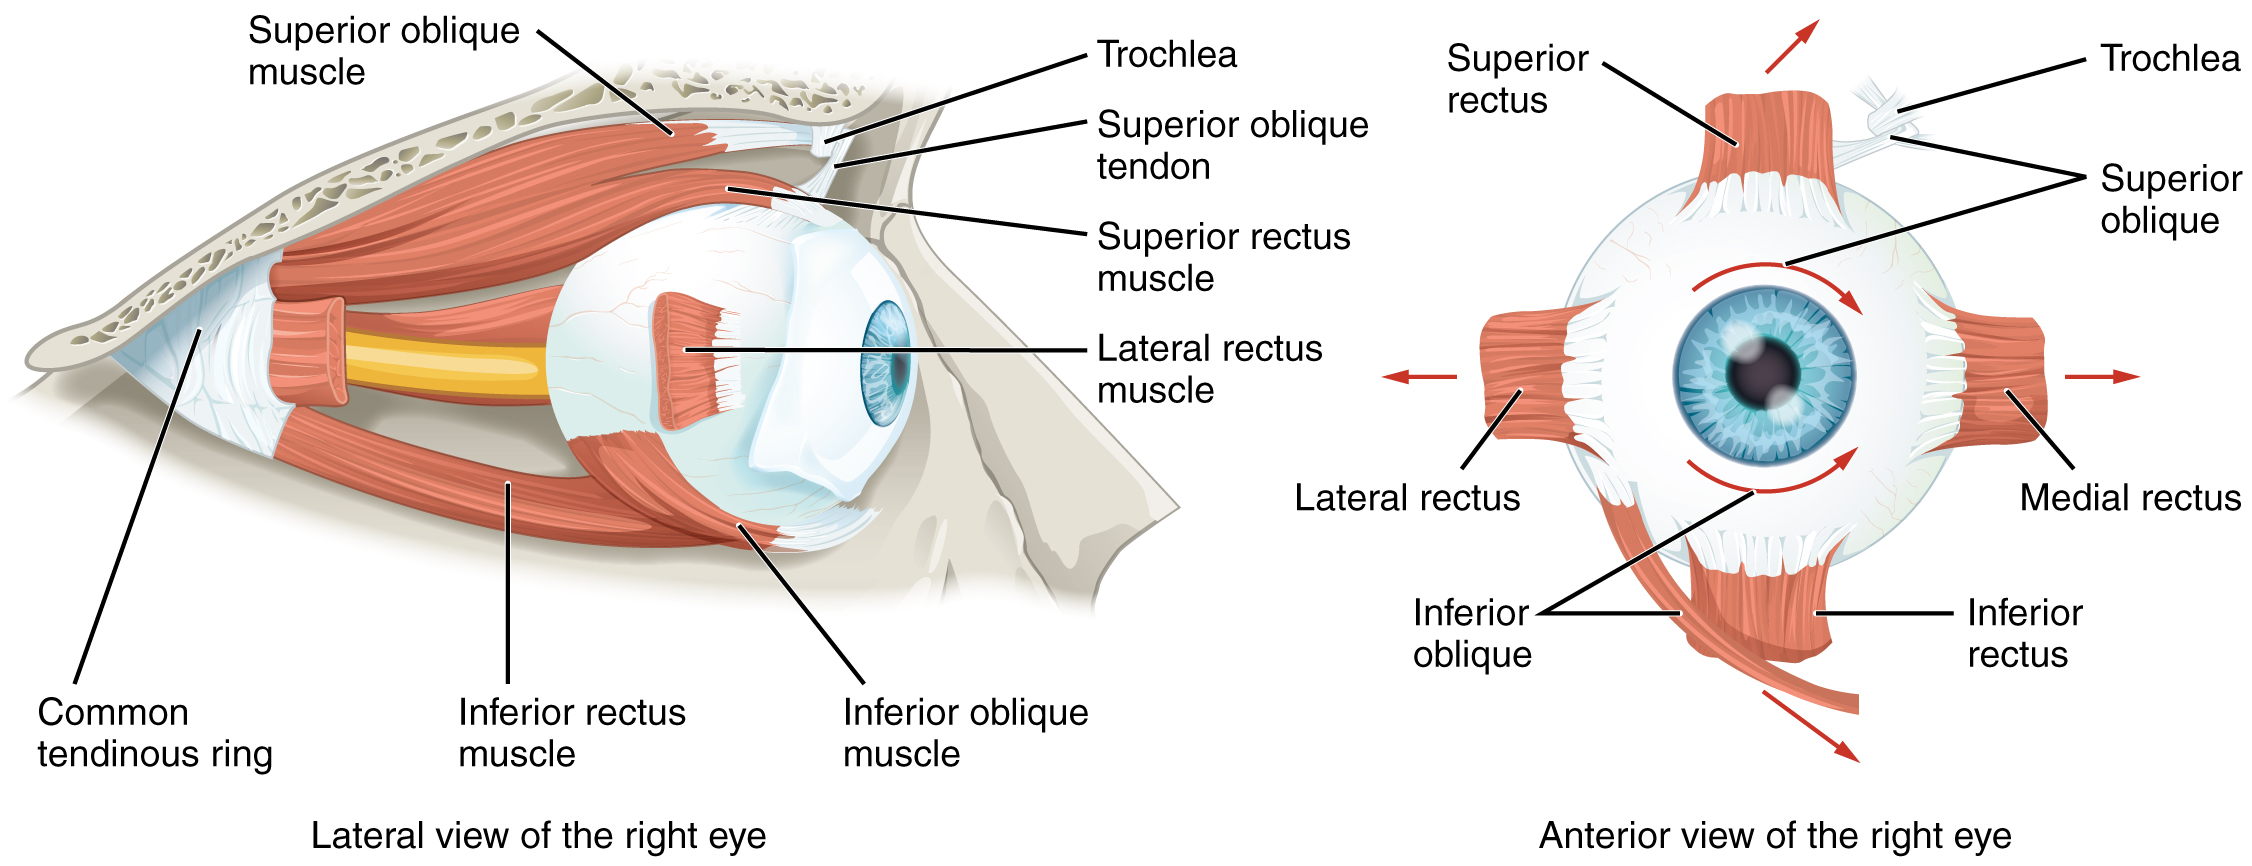
\includegraphics[width=0.95\textwidth]{images/extraocularMuscles.jpg}
\caption{Músculos extraoculares. Crédito de imagen: OpenStax
  \cite{openStax2017sensory}, licensia Creative Commons Attribution
  (CC BY).}
\label{fig:eyeMuscles}
\end{figure}

\subsection*{Medir los movimientos oculares producidos por los músculos oculares}

Idealmente, nos gustaría registrar la actividad de los músculos
extraoculares usando electromiografía (EMG). Sin embargo, como vimos
en la práctica `Fundamentos de la Electromiografía', registros no
invasivos (con electrodos de superficie) son difíciles de obtener de
algunos músculos, especialmente si los músculos no están ubicados
superficialmente, sino en capas más profundas. Los músculos
extraoculares se encuentran dentro de la cuenca del ojo y encima de
ellos se encuentran músculos faciales como el obicularis oculi, que
controlar los movimientos de los párpados. Por lo tanto, es probable
que cualquier registro EMG de superficie que intentamos alrededor del
ojo detectaría actividad de estos músculos, en lugar de nuestros
músculos de interés. Por lo tanto, necesitamos encontrar otra
forma de registrar los movimientos oculares. Afortunadamente, otras
propiedades eléctricas del ojo proporcionan tal alternativa.

%While the extraocular muscles have the same striated structure and
%the same contraction mechanisms as typical skeletal muscle, there are
%important differences. For example, while many skeletal muscle motor
%units are silent at rest, motor units of the eye show high levels of
%baseline activity. This tonic firing is in the range of 100-150 Hz,
%and is so pronounced that some have said there is really ``no
%position of rest for extraocular muscles"
%\cite{breinin1955electromyography}. Thus, what we will be looking for
%as an indication of muscle activation associated with eye movement
%will not be the beginning of firing after a period of quiescence, as
%with a bicep or similar, but rather a dramatic increase in the firing
%rate. To overcome the viscous forces opposing saccadic-type movements
%in the eye, extraocular motor units will show bursts of rapid firing
%as high as 600 Hz. The firing rate decreases again when the eye
%reaches the new position.

\subsection*{Dipolo eléctrico}
Un dipolo eléctrico está formado por dos cargas de signo opuesto,
$q^+$ y $q^-$, separados por una distancia, $d$
\cite{hyperphysicsDipole}. El momento dipolar eléctrico es un vector,
$\vec{p}$, dado por el producto de la magnitud de la carga, $q$, y la
distancia entre las dos cargas. Por convención, el vector se apunta
desde la carga negativa hacia la positiva (Fig. \ref{fig:dipole}).

\begin{figure}[h!]
\centering
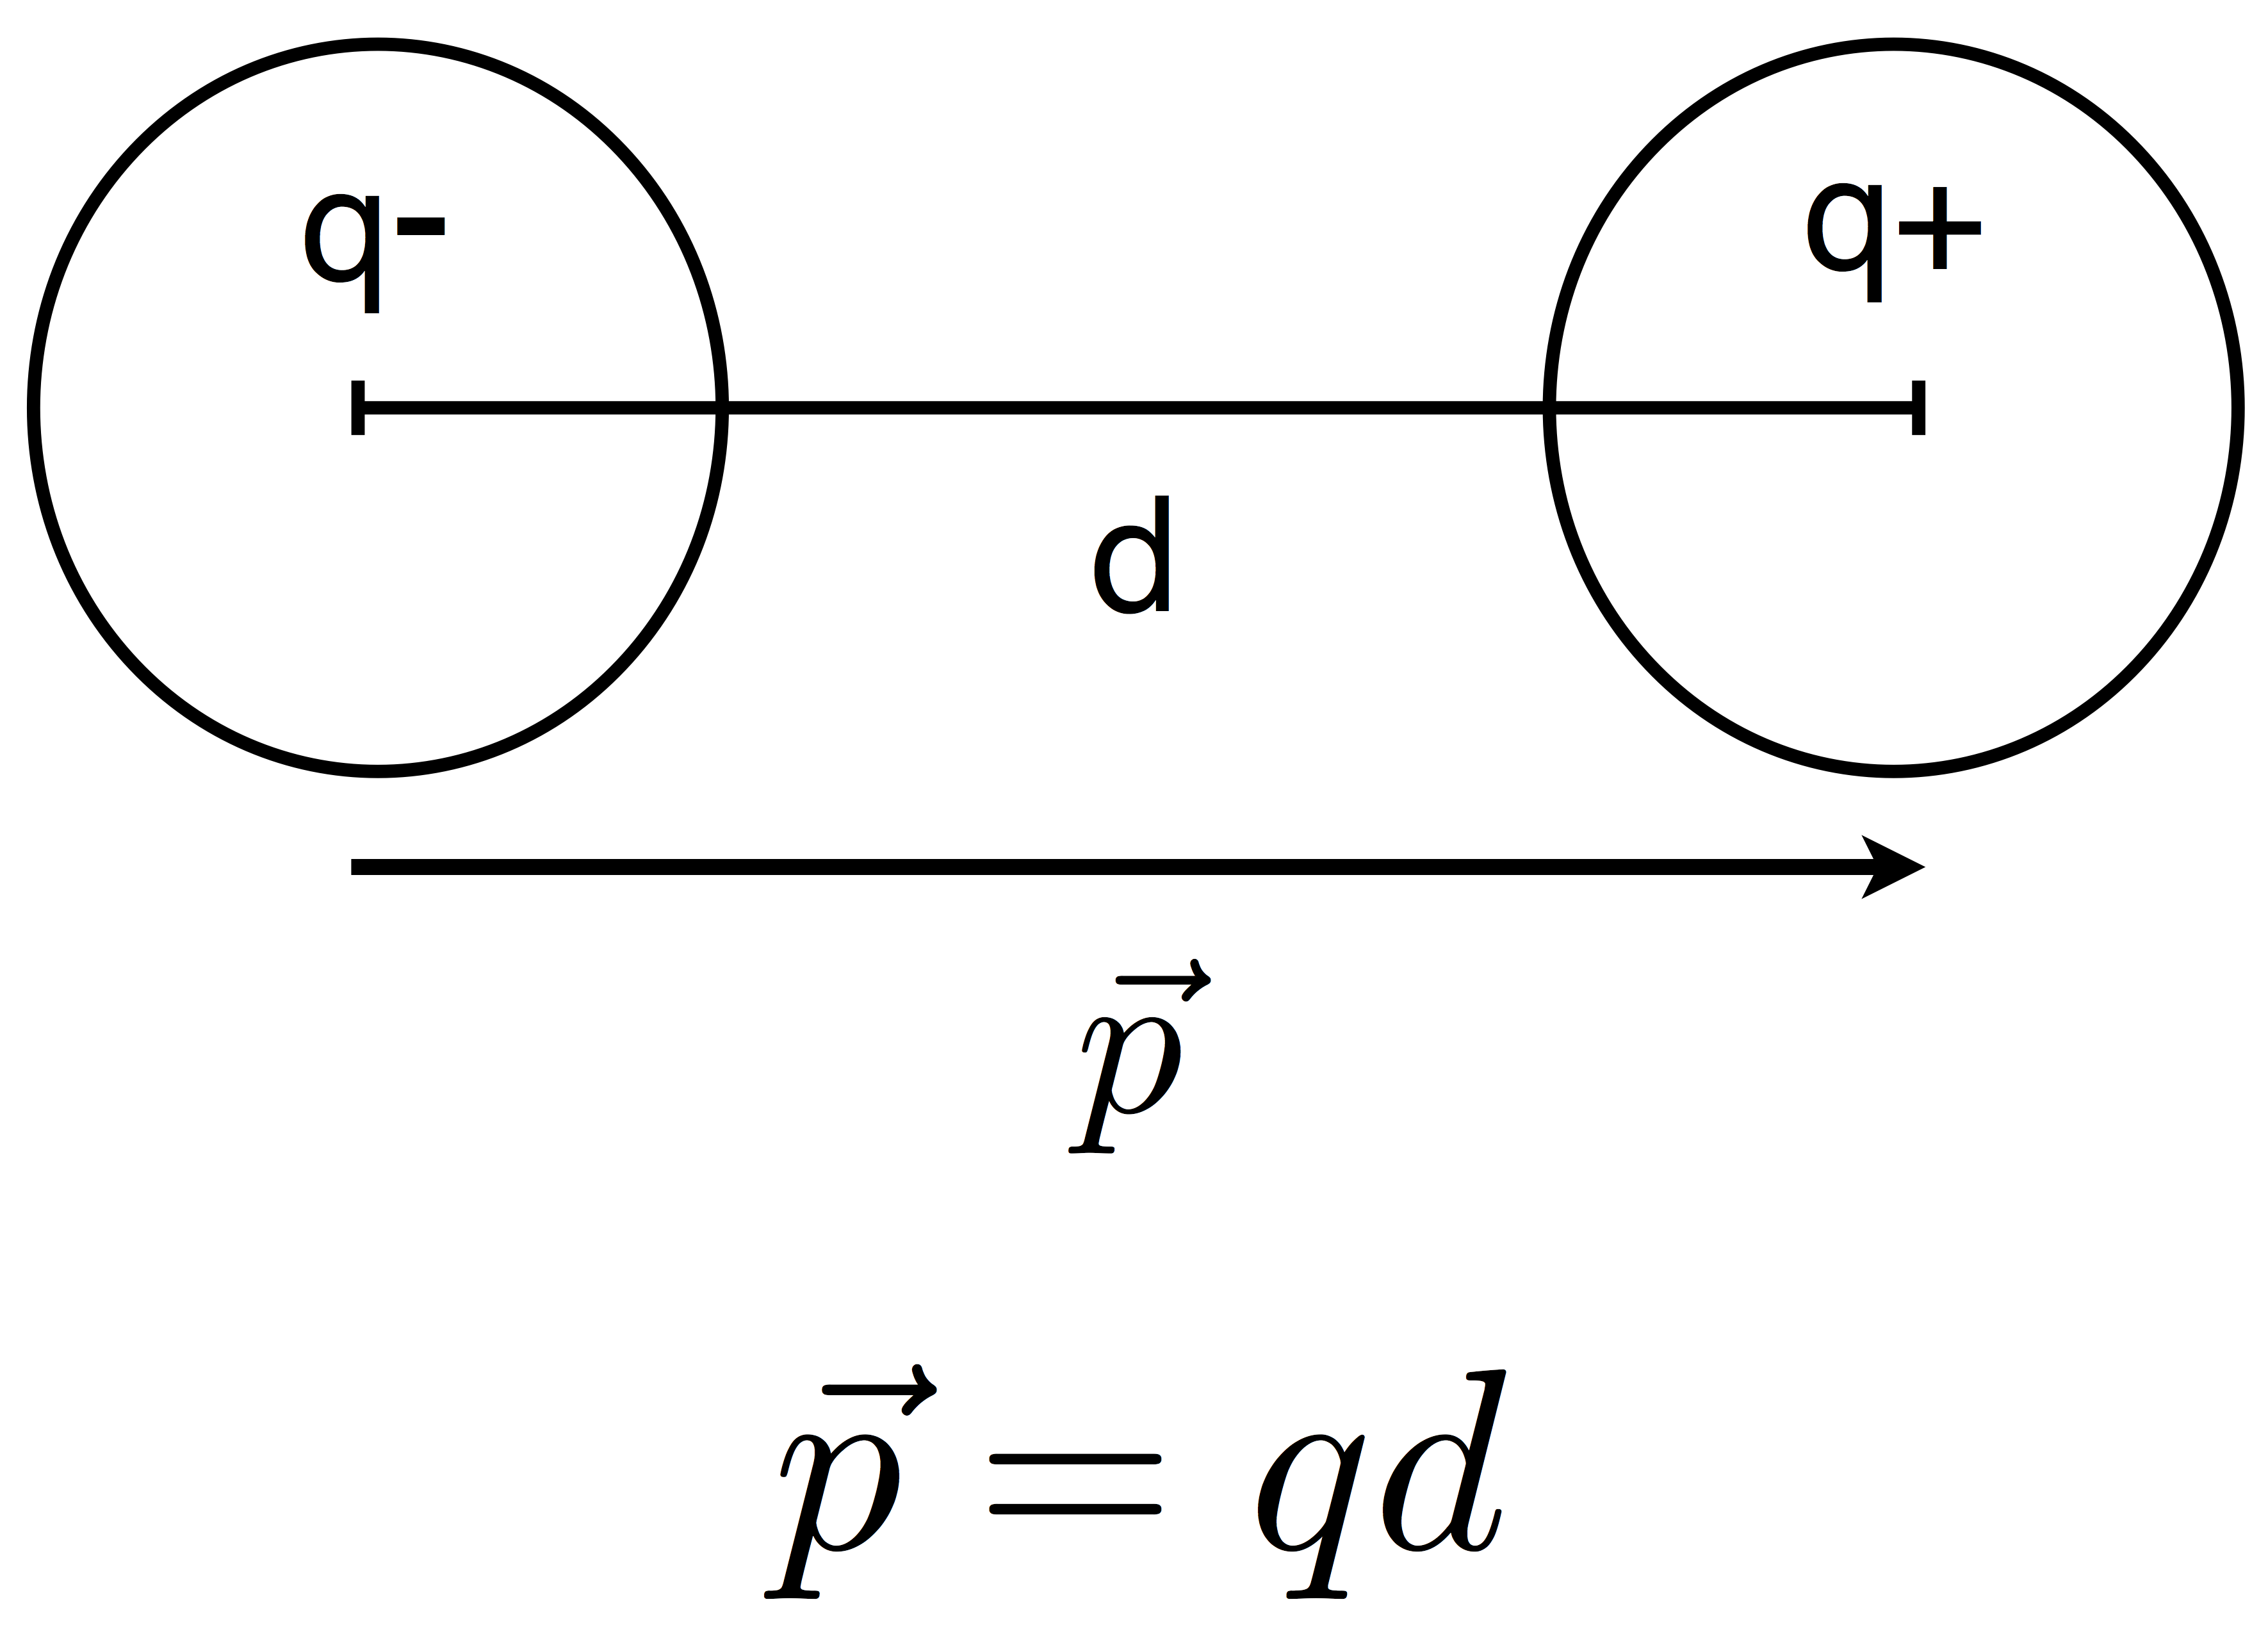
\includegraphics[width=0.5\textwidth]{images/dipole.png}
\caption{Representación esquemática de un dipolo eléctrico. Crédito de
  imagen: Erin C. McKiernan, CC BY.}
\label{fig:dipole}
\end{figure}

\subsection*{Dipolo del ojo}
Existe una diferencia de potencial entre la córnea y la retina,
llamado potencial corneoretinal (CRP por sus siglas en inglés) o el
\emck{standing potential} del ojo
\cite{heide1999electrooculography,marg1951development,malmivuo1995bioelectromagnetism}. La
córnea es positiva en relación con el potencial negativo en la retina,
estableciendo así un dipolo eléctrico que apunta desde la parte
posterior a la frente del ojo (Fig. \ref{fig:crp}). El movimiento del
ojo causará que el dipolo se mueve y cambia el campo eléctrico
circundante \emck{surrounding}. Como veremos, podemos medir estos
cambios con la electrooculograma.

\begin{figure}[h!]
\centering
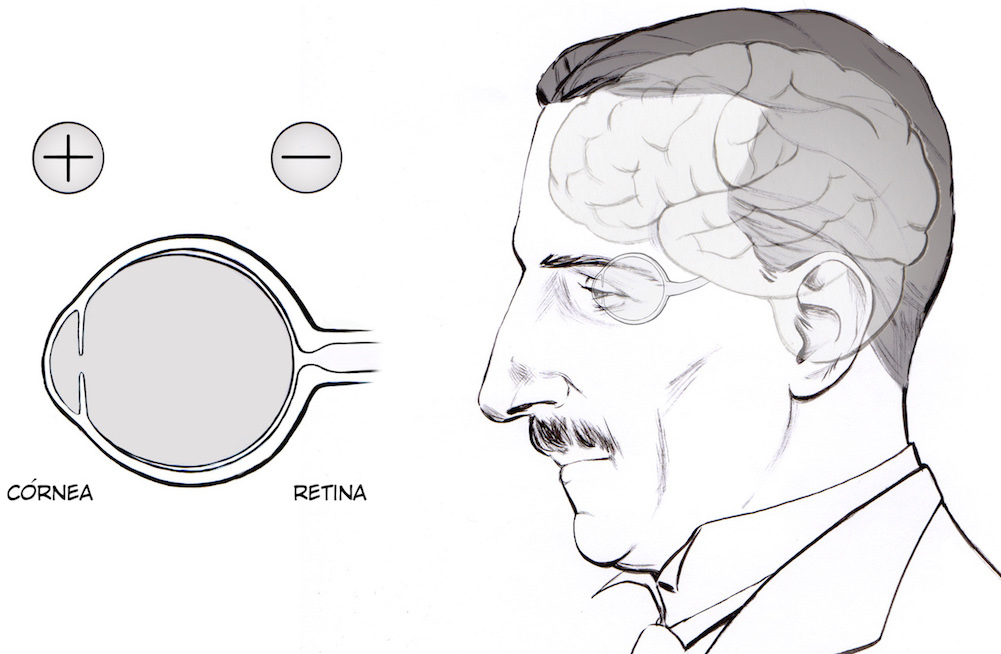
\includegraphics[width=0.7\textwidth]{images/eyePolarity.jpg}
\caption{El dipolo eléctrico del ojo. Credito de imagen: Backyard
  Brains, CC BY-SA.}
\label{fig:crp}
\end{figure}

El \emck{standing potential} del ojo se debe en gran parte a la
diferencia en potencial a tráves del epitelio pigmentario de la retina
(RPE) \cite{heide1999electrooculography,berg1991dipole}, el potencial
transepitelial (TEP). El TEP se establece y se mantiene por el
transporte de iones a través de las membranas apical y basolateral de
las células epiteliales \cite{joseph1991apical,quinn1992ion}.

Este transporte se lleva a cabo mediante proteínas transmembranales
especializadas conocidas como canales iónicos y bombas
\cite{khanTransport}. Los canales iónicos se abren a permitir que los
iones fluyan hacia dentro o fuera de la célula con su gradiente
electroquímico. Las bombas vienen en una variedad de tipos, incluyendo
simportadores que co-transportan iones en la misma dirección e
intercambiadores que traen un ion hacia adentro y envian otro ion
hacia afuera. Las bombas pueden usar ATP directamente o indirectamente
para transportar iones en contra de sus gradientes electroquímicos
\cite{khanTransport}.

Cualquier cambio en el transporte iónico a través de la capa epitelial
alterará el TEP y, a su vez, se refleja en el CRP registrado a través
de la electrooculograma (EOG). La amplitud del CRP registrado en el
EOG típicamente varia entre cientos de microvoltios ($\mu$ V) a un
milivoltio (mV). El TEP varía con condiciones de luz y oscuridad
\cite{heide1999electrooculography}.

\subsection*{Electrooculograma}
La electrooculografía mide los cambios en el dipolo eléctrico del ojo
y los registros que obtenemos se llaman electrooculogramas (EOGs)
\cite{heide1999electrooculography,marg1951development,malmivuo1995bioelectromagnetism}. Similar
a lo que vimos en la práctica de ``Los Fundamentos de la
Electromiografía'', la EOG es un registro diferencial en lo cual
colocamos dos electrodos, restando las señales registradas en los dos
puntos, y luego amplifica la diferencia. Cuando los ojos están en la
posición de descanso, mirando directo, los electrodos no registran
ninguna diferencia en potencial. Sin embargo, cuando los ojos se
mueven en una dirección dada, el extremo positivo del dipolo se mueve
más cerca de un electrodo y más lejos del otro. Dado que estamos
midiendo la diferencia entre los potenciales registrados en los dos
electrodos, esto dará como resultado una deflexión positiva cuando los
ojos se mueven en una dirección y una desviación negativa cuando se
mueven en la otra dirección \cite{malmivuo1995bioelectromagnetism}
(Fig. \ref{fig:eog}).

\vspace{0.5cm}

\textbf{Preguntas de estudio:}

\begin{itemize}
\item ¿Cómo colocarán sus electrodos para registrar la elevación y
  depresión del ojo?
\item ¿Cómo colocarán sus electrodos para registrar la aducción y
  abducción del ojo?
\end{itemize} 

\begin{figure}[t!]
\centering
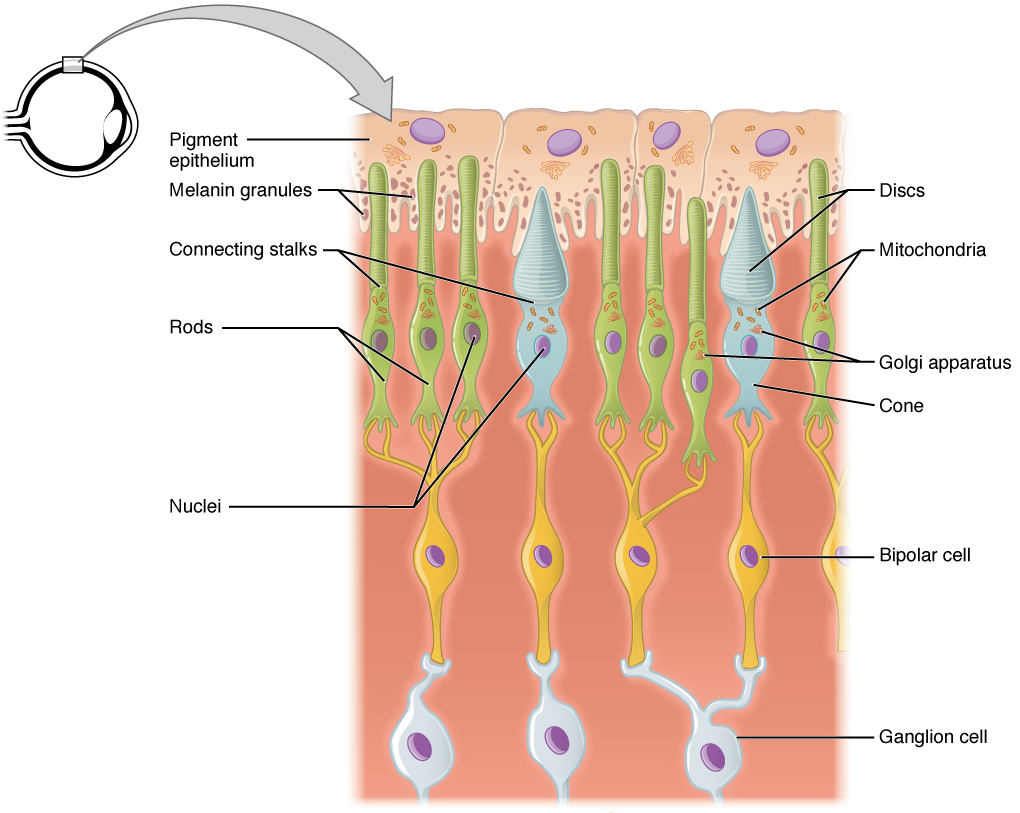
\includegraphics[width=0.81\textwidth]{images/rpe.png}
\caption{Organización del ojo que muestra el epitelio pigmentario de
  la retina (RPE). Credito de imagen: OpenStax
  \cite{openStax2017sensory} }
\label{fig:rpe}
\end{figure}

\begin{figure}[b!]
\centering
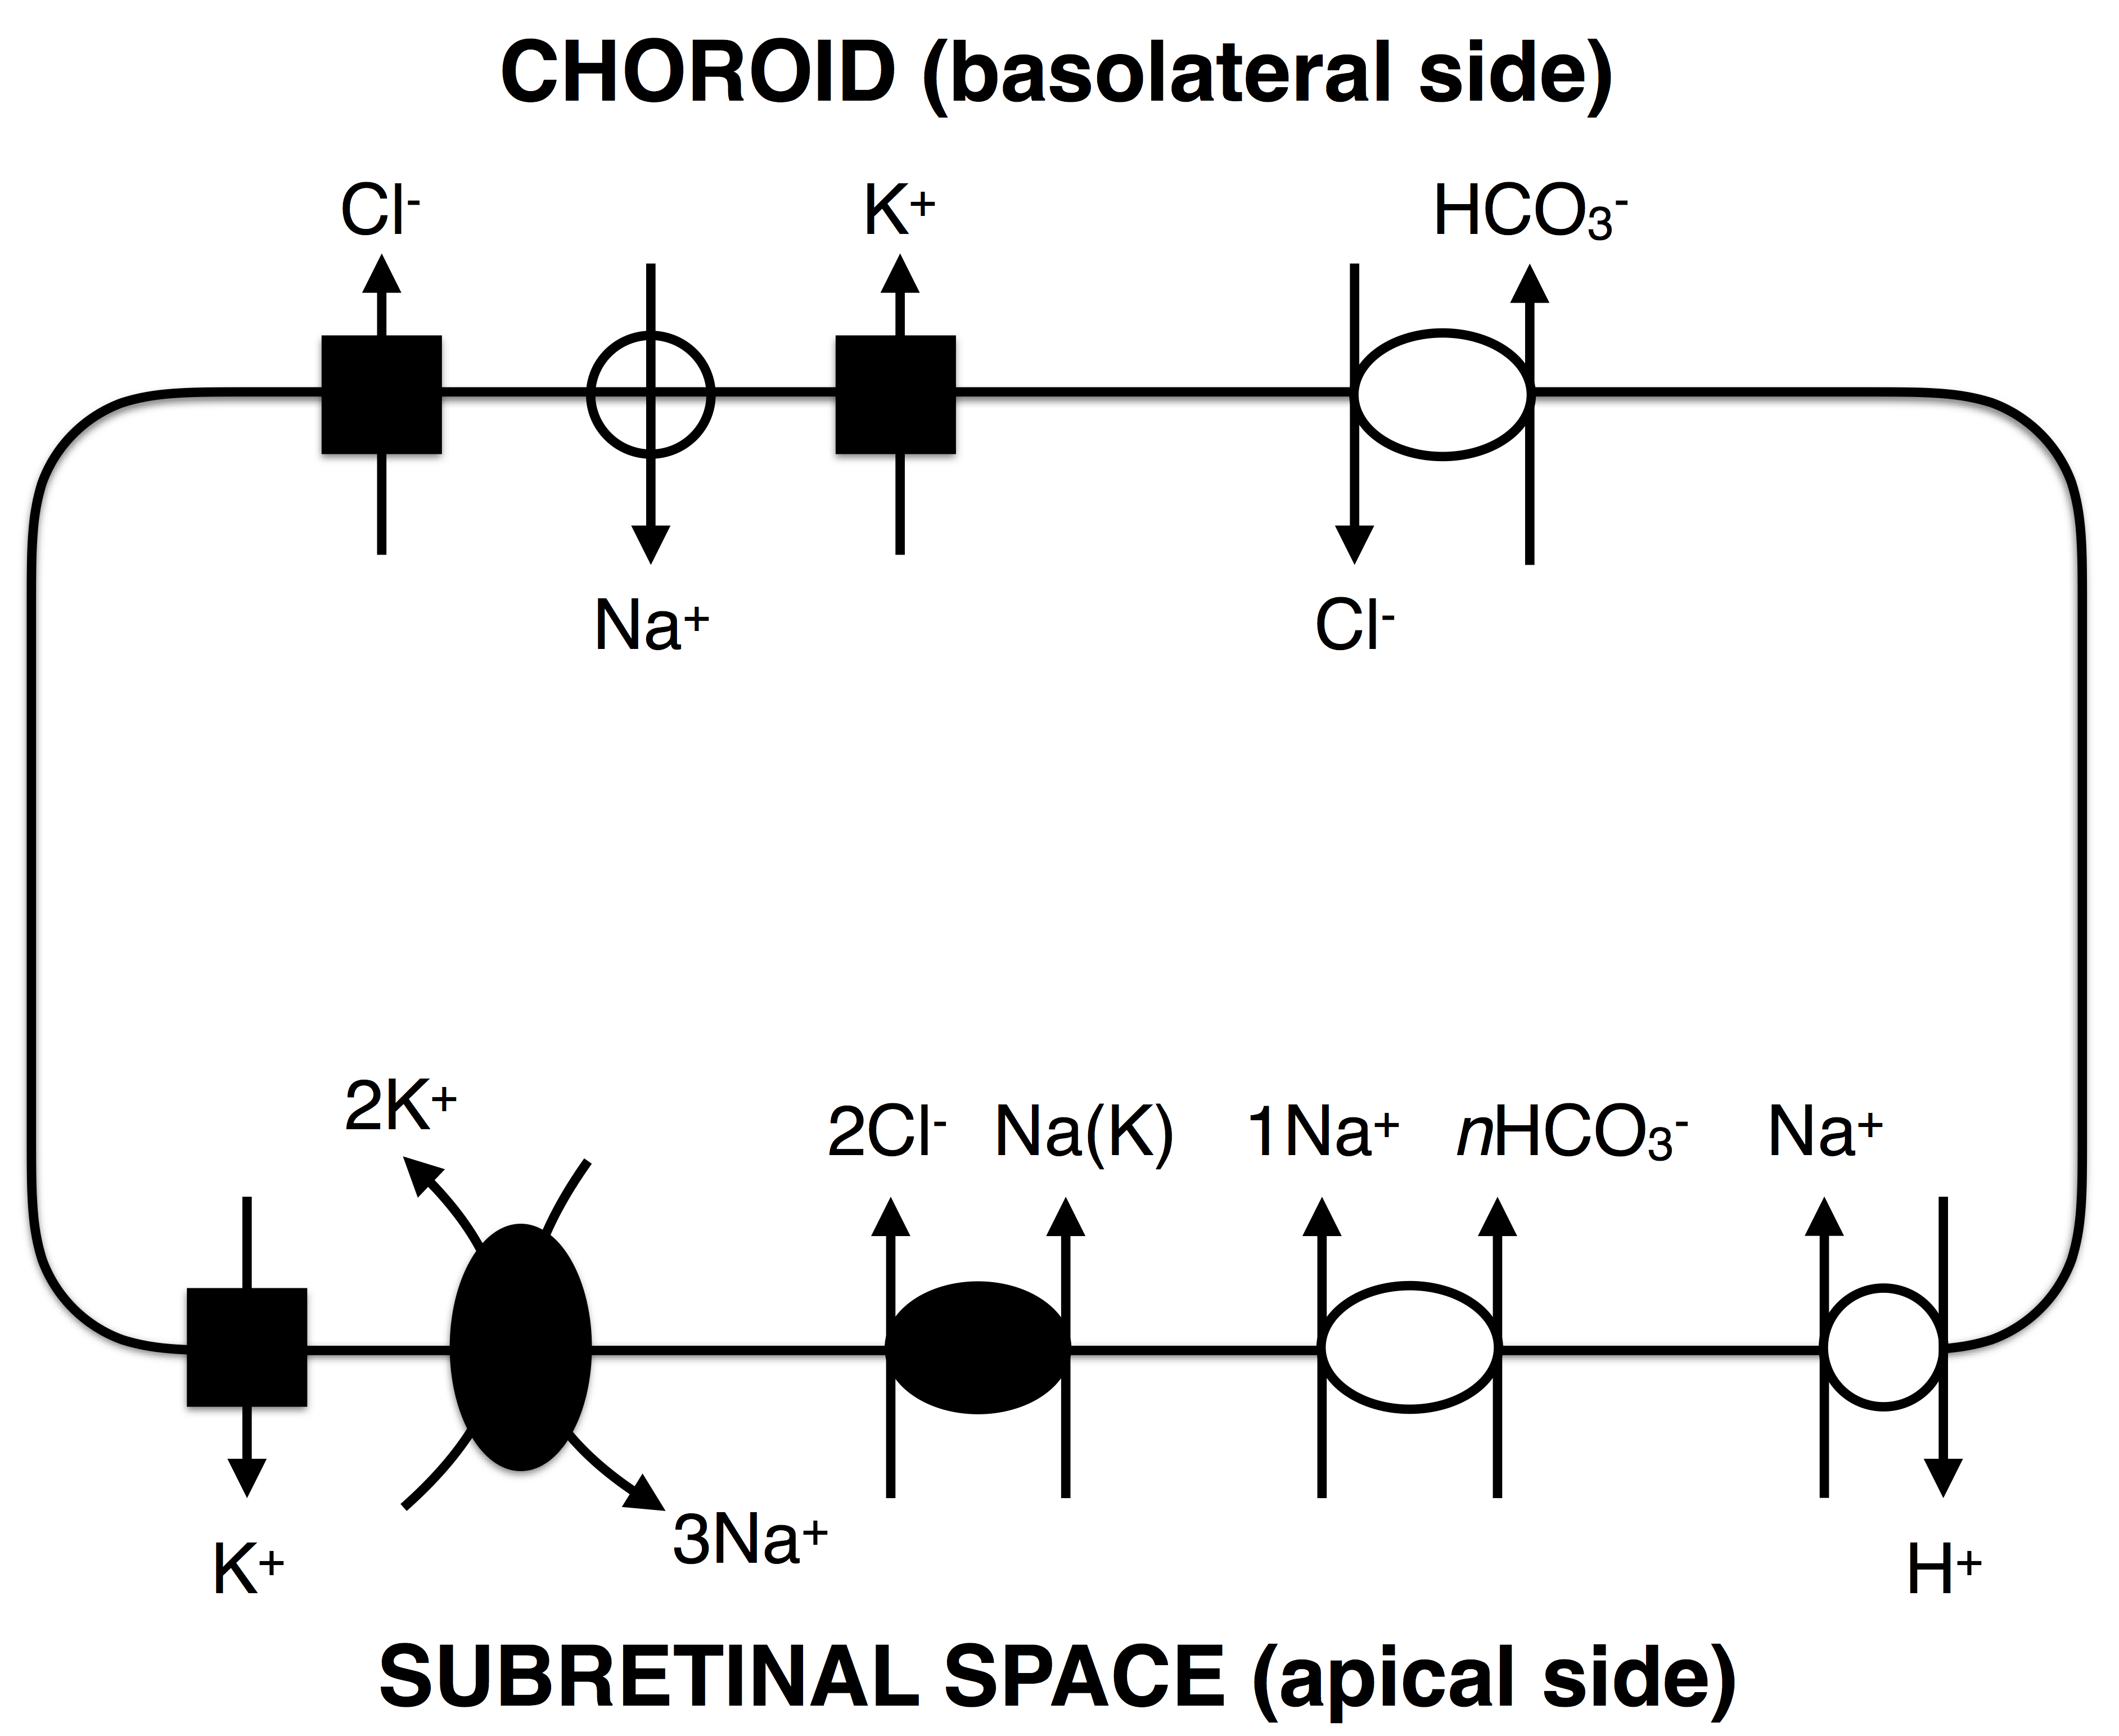
\includegraphics[width=0.63\textwidth]{images/rpeTransport.png}
\caption{Transporte de iones a través de canales y bombas en el
  RPE. Credito de imagen: Erin C. McKiernan, CC BY. Basado en
  información en \cite{joseph1991apical,quinn1992ion}}
\label{fig:crp}
\end{figure}

\begin{figure}[h!]
\centering
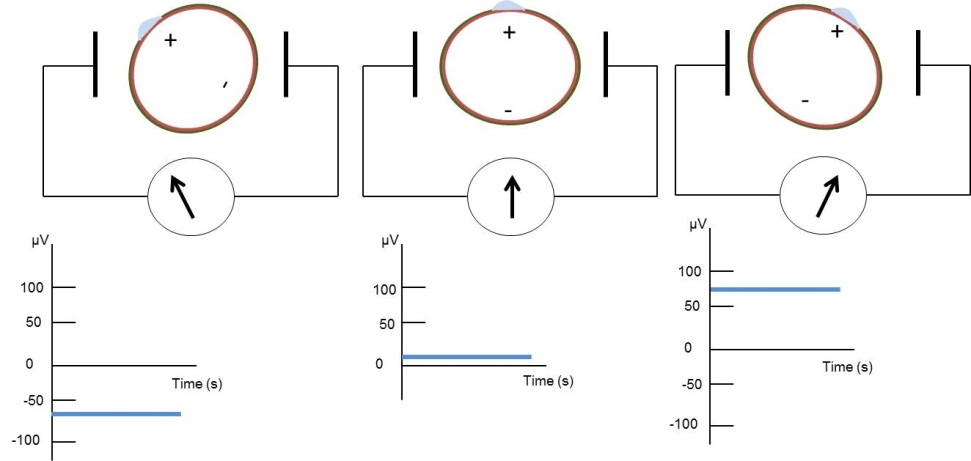
\includegraphics[width=0.95\textwidth]{images/eog.jpeg}
\caption{Esquema de un registro EOG. Las gráficas superiores muestran
  la posición del ojo y su dipolo, mientras que las gráficas
  inferiores muestran los registros EOG en microvoltios. En la
  posición de descanso (columna central), el dipolo eléctrico del ojo
  está orientado hacia adelante y se registra poca o ninguna
  diferencia de potencial entre los dos electrodos. Cuando los ojos se
  mueven hacia la izquierda (columna izquierda), el extremo positivo
  del dipolo se mueve hacia el electrodo izquierdo y produce una
  deflexión negativa en el EOG. Cuando los ojos se mueven hacia la
  derecha (columna derecha) el extremo positivo del dipolo se mueve
  hacia el electrodo derecho y produce una deflexión positiva en el
  EOG. Crédito de imagen: \cite{viqueira2013ocular}}
\label{fig:eog}
\end{figure}

\section*{PROCEDIMIENTO}
Antes de comenzar, asegúrese de tener todo el equipo necesario y tener
instalado el software de grabación en su computadora o teléfono
inteligente. El equipo Backyard Brains viene ensamblado y listo para
registrar. Los siguientes pasos lo guiarán en el montaje del equipo y
llevando a cabo los registros.

\subsection*{1. Configurar registros EOG}

\begin{enumerate}
\item Conecte la pila de 9V a sus terminales en el Heart and Brain
  SpikerShield Box
\item Conecte el cable USB azul al puerto Arduino en el Heart and
  Brain SpikerShield Box
\item Conecte el otro extremo del cable USB a su computadora
\item Conecte el cable naranja a su puerto correspondiente en el Heart
  and Brain SpikerShield Box
\item Coloque los electrodos de superficie para registrar primero la
  elevación y depresión del ojo, con un electrodo de superficie sobre
  el ojo y otro debajo (Fig. \ref{fig:ePlacement}A,B). Luego, registre
  la aducción y abducción, con un electrodo de superficie a la
  izquierda del ojo izquierdo y uno a la derecha del ojo derecho
  (Fig. \ref{fig:ePlacement}C)
\item El electrodo de referencia debe colocarse detrás de una oreja,
  justo sobre el proceso mastoideo (Fig. \ref{fig:ePlacement}A,D)

\vspace{0.2cm}

\begin{figure}[h!]
\centering
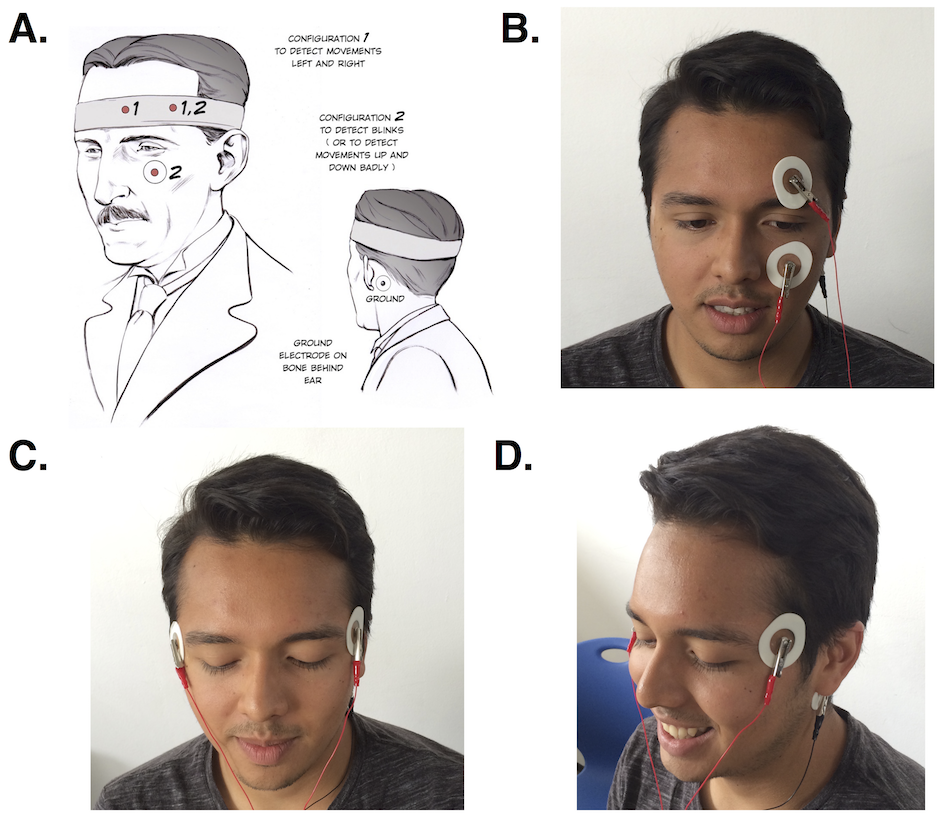
\includegraphics[width=0.9\textwidth]{images/eogElectrodes.png}
\caption{A. Dibujos mostrando dos posibles ubicaciones de
  electrodos. Crédito de imagen: Backyard Brains, CC
  BY-SA. B,C. Colocación de electrodos para registrar elevación y
  depresión (B.) o aducción y abducción (C). D. Colocación del
  electrodo de referencia. Créditos de imagenes: B-D: Erin McKiernan,
  CC BY.}
\label{fig:ePlacement}
\end{figure}

\item Conecte cada una de las pinzas de cocodrilo rojas en el extremo del
  cable naranja a uno de los electrodos de superficie; asegúrese de
  que los clips metálicos no se toquen y trate de evitar enredar los
  cables
\item Conecte el clip de cocodrilo negro (referencia) al electrodo
  colocado detrás de la oreja
\item To improve the EMG signal, the area where the electrodes will be
  placed can be cleaned with alcohol prior to placement; wait until
  the area is dry to place the electrodes
\item Para mejorar la señal EOG, el área donde los electrodos serán
  colocados puede limpiarse con alcohol antes de la colocación; esperar
  hasta el área está seca para colocar los electrodos
\item El gel de electrodos se puede aplicar para mejorar la
  conducción, pero muchas veces no es necesario
\item Para evitar artefactos de ruido, asegúrese de que ninguna prenda
  de ropa toque los electrodos o cepillar contra \emck{brush against?}
  los cables durante el registro
\end{enumerate}

\subsection*{2. Poner a prueba los registros EOG}

\begin{enumerate}
\item El Heart and Brain SpikerShield Box se encenderá automáticamente
  cuando está conectado a la computadora, indicado por la luz verde
\item Abra el software de grabación de Backyard Brains y explore los
  controles y configuraciones (para obtener más información sobre el
  uso del software, consulte [\cite{spikeRecorder}])
\item Pídale al sujeto que mueva brevemente sus ojos y verifique que
 se ve una desviación correspondiente en el registro
\item Intente guardar un registro de prueba en su computadora (el
  formato será .wav)
\end{enumerate}

\subsection*{3. Coleccionar los datos}

\begin{enumerate}
\item Asegúrese de que el sujeto esté en una posición de descanso con
  los ojos hacia adelante
\item Cuando el sujeto esté listo, presione registrar en la interfaz
  de software de Backyard Brains
\item Indique al sujeto que permanezca relajado durante 3-5 segundos
  después de que comienza la grabación, luego muoverse los ojos hacia
  arriba para registrar la elevación
\item Luego, pida al sujeto que regrese a la posición de descanso para
  3-5 segundos
\item Luego, instruya \emck{instruct} al sujeto mover sus
  ojos hacia abajo para registrar depresión ocular
\item Pida al sujeto que repita la secuencia anterior 3 veces
\item Termine la grabación y guarde los datos en su computadora
\item Comience un nuevo registro para examinar el efecto del tamaño
  del movimiento del ojo
\item Para ayudar al sujeto a hacer movimientos oculares de diferente
  magnitudes, coloque su dedo en 3 alturas diferentes arriba o abajo
  el ojo para servir como nuevos puntos de fijación
\item Termine la grabación y guarde los datos en su computadora
\item EOG debe guardarse y exportarse en formato .wav para su análisis
\item Cambiar la colocación del electrodo para registrar aducción y
  abducción y repita los pasos 1-11
\end{enumerate}

\section*{ACKNOWLEDGMENTS}
Este trabajo fue apoyado por la Dirección General de Asuntos del
Personal Académico, Programa de Apoyo a Proyectos para la Innovación y
Mejoramiento de la Enseñanza en la Universidad Nacional Autónoma de
MéXico (UNAM-DGAPA-PAPIME clave PE213817).

\newpage
 
% BIBLIOGRAPHY
\begin{small}
\bibliography{eye}
\end{small}

\end{document}
